% Created 2017-02-20 Mon 10:10
\documentclass[11pt]{article}
\usepackage[utf8]{inputenc}
\usepackage[T1]{fontenc}
\usepackage{fixltx2e}
\usepackage{graphicx}
\usepackage{grffile}
\usepackage{longtable}
\usepackage{wrapfig}
\usepackage{rotating}
\usepackage[normalem]{ulem}
\usepackage{amsmath}
\usepackage{textcomp}
\usepackage{amssymb}
\usepackage{capt-of}
\usepackage{hyperref}
\author{Pedro Cunial}
\date{\today}
\title{Pesquisa 05 -- Kit de Desenvolvimento SAME-70}
\hypersetup{
 pdfauthor={Pedro Cunial},
 pdftitle={Pesquisa 05 -- Kit de Desenvolvimento SAME-70},
 pdfkeywords={},
 pdfsubject={},
 pdfcreator={Emacs 25.1.1 (Org mode 8.3.6)},
 pdflang={English}}
\begin{document}

\maketitle
\tableofcontents


\section{Overview}
\label{sec:orgheadline2}
\subsection{Esboce um diagrama de blocos que ilustre a interação entre o uC, hardware, firmware}
\label{sec:orgheadline1}
O uC serve como ponto central da execução de u firmware em um hardware. O firmware é colocado no uC, o qual o executa no hardware.

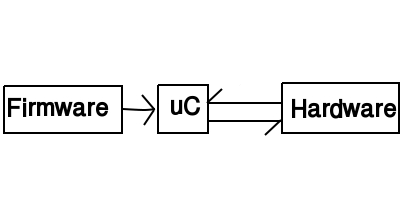
\includegraphics[width=\textwidth]{diagrama}

\section{SAM-E70 microcontrolador}
\label{sec:orgheadline3}
  \subsection{Identifique a família e liste as especificidades do
    microcontrolador utilizado no curso}
\label{sec:orgheadline4}
  O microcontrolador utilizado no curso é o SAM E70, um uC baseado no chip ARM
  32-bits Cortex-M7, que segue o padrão de arquitetura RISC. Ele opera no máximo
  sob o clock de 300MHz e possui uma unidade de ponto flutuante (FPU).

  Além disso, o uC possui uma memória externa Flash de 2048KB, dois caches de
  16KB e até 384KB de SRAM (podendo variar de acordo com a versão). O uC pode
  ter uma variedade de números de pinos, definidos pela sua versão.

  \subsection{Liste os tipos de memórias internas do microcontrolador
    SAM-E70 e seus tamanhos}
\label{sec:orgheadline4}
  Como mencionado anteriormente, o SAM-E70 possui uma memória Flash externa de
  2048KB, dois caches de 16KB cada e uma memória SRAM de até 384KB, dependendo
  da versão do uC.

  \subsection{Por que é importante saber quanto de memória um uC
    possui?}
\label{sec:orgheadline4}
  É importante a noção do tamanho da memória de um uC na projeção de um projeto,
  sendo este um fator limitante na decisão de algoritmos e otimizações. Além do
  que, o tamanho da memória onde o firmware será escrito pode limitar o tamanho
  do mesmo.

  \subsection{Escolha um dos periféricos do uC e explique sua funcionalidade}
\label{sec:orgheadline4}
  O TRNG, ou True Random Number Generator, é um periférico que se baseia em
  fenômenos físicos (não computacionais) para a geração de números aleatórios.

  Este periférico costuma ser baseado em fenômenos que geram ruídos de baixa
  intensidade no uC, como ``ruídos térmicos'', efeitos foto-elétricos ou até
  mesmo processamentos quanticos.

  \subsection{O que é watchdog timer e qual é sua utilização?}
\label{sec:orgheadline4}
  O watchdog timer é um periférico que ``vigia'' o processador de um computador
  para garantir que ele de fato está funcionando, podendo detectar e recuperá-lo
  caso contrário.

  \subsection{Pesquise nos fornecedores qual o valor de mercado do chip
    utilizado no kit de desenvolvimento SAM-E70}
\label{sec:orgheadline4}
  Os processadores da família ARM Cortex-M7 costumam estar na faixa entre 10 e
  15 dolares, podendo variar de acordo com a sua versão mais específica e ano de fabricação.

  \section{SAM-E70-XPLD hardware}
\label{sec:orgheadline4}
  \subsection{Descreva como funciona a gravação via JTAG e porquê é
    bastante utilizada pela industria}
\label{sec:orgheadline4}
  Na gravação de um dispositivo utilizando JTAG, quatro linhas seriais são
  acessadas, a TMS, TCK, TDI e TDO, permitindo rápido acesso à portas, memória,
  lock bits, registradores e outros fatores do chip.

  O principal motivo de adoção do JTAG pela industria se da pela padronização
  dos programadores do tipo, permitindo maior compatibilidade e reuso do
  material entre diferentes produtos.

  \subsection{Qual a relação do clock no consumo de energia em sistems eletrônicos?}
\label{sec:orgheadline4}
  Quanto maior o clock de um dispositivo, maior a quantidade de operações que o
  mesmo realiza por segundo e, consequentemente, maior o gasto de energia do
  mesmo.

  Em dispositivos embarcados é comum a utilização de ``underclock'', reduzindo o
  clock de um uP em busca de melhor aproveitamento da energia. A comunidade
  entusiasta de Android e suas builds alternativas têm produzido muito material
  e maneiras de auxílio para o ``underclock'' de seus dispositivos justamente
  com o intuito de aumentar a duração da bateria por carga.

  \subsection{Qual o valor do cristall utilizado no kit SAME-70?}
\label{sec:orgheadline4}
  O SAME-70 possui um oscilador interno RC com uma frequência que pode variar de
  4 à 12 MHz, sendo o seu padrão de fábrica 4MHz, além de um cristal externo
  de 32.768 kHz ou um embarcado RC de 32 kHz (mais comum).

  \section{Firmware -- Especificidades}
  \subsection{O que são variáveis volatile/const/static?}
\label{sec:orgheadline4}
  O qualifier ``volatile'' indica ao compilador que o valor de uma dada variável
  pode mudar à qualquer momento, mesmo sem ser explicitado no programa, ou seja,
  na grande maioria das vezes, é uma variável que pode ser alterada por um
  programa externo e que não deve ser otimizada pelo compilador.

  O qualificador ``const'' especifica que uma variável deve ser alocada na
  memória e nunca mais deverá mudar. Isso pode ser útil principalmente para a
  alocação de strings, uma vez que ao utilizar o #define, cada vez que a string
  for instanciada um novo valor da mesma será alocado.

  Por fim, o qualificador ``static'' faz com que uma variável dentro de uma
  função mantenha seu valor entre diferentes chamadas da mesma, além de ser
  visivel somente dentro do arquivo no qual fora declarada (o mesmo vale para
  funções ``static'').

  \subsection{O que é um makefile e qual a sua utilização?}
\label{sec:orgheadline4}
  Um makefile é um arquivo para a compilação de um dado projeto (normalmente em
  C/C++). A principal vantagem de utilizar uma Makefile ao invés de simplesmente
  re-compilar um código na linha de comando é que a Makefile pode evitar
  ``compilações redundantes'', ou seja, compilar arquivos que suas saídas já
  existem e não precisariam ser recompilados. Além disso, é possível escrever
  diversos scripts dentro de um Makefile, como um de instalação, um de
  compilação, um de desinstalação etc.

  \subsection{O que é ASCII e quando é utilizado?}
\label{sec:orgheadline4}
  A tabela ASCII é uma tabela que define os valores para cada possível valor de
  um char em uma representação gráfica (onde os principais valores utilizados
  costumam ser letras, mas isso não é necessariamente sempre verdade). A tabela
  ASCII é utilizada sempre que representamos um ``char'' como string no print em
  linguagens de mais baixo nível como C. Existe também o padrão UTF-8, que
  pretende expandir a tabela ASCII, mas que exige um maior número de bits por
  caracter e por isso não é tão utilizado como o ASCII.

  O ASCII foi de extrema importância na computação pois padronizou a maneira com
  que caractéres deveriam ser representados em bits, tornando-se o principal
  padrão do mesmo.

  Por fim, vale lembrar que a representação de um caractér seguindo a tabela
  ASCII é apenas uma convensão e que um char que vale 65 não necessariamente
  precisa representar a letra 'A'.

\end{document}